\section{Evaluation}
\label{chap:evaluation}
Am Ende unserer Arbeit wurde uns ein Framework des SAFEST-Projekts zur Verfügung gestellt, dass die Möglichkeit bietet, verschiedene vorimplementierte Algorithmen mit einander zu vergleichen.\\
Nachdem wir unseren Algorithmus in das Framework integriert hatten, haben die folgenden Vergleiche mit einer vorimplementierten, Histogramm-basierten Lösung angestellt:
\begin{itemize}
	\item[a)] die vorimplementierte Lösung, die mit Histogrammen arbeitet
	\item[b)] unsere HMM-basierte Lösung mit generischen Werten für Initialwerte, Emission und Transition ohne Lernen
	\item[c)] unsere HMM-basierte Lösung mit generischen Werten für Initialwerte, Emission und Transition mit Lernen
\end{itemize}
Weitere Vergleiche haben wir nicht angestellt, da das Histogramm-basierte Verfahren den anderen Verfahren entweder überlegen ist (OpenCV MOG und OpenCV MOG2) oder aber das Verfahren den Hintergrund hart auf bestimmte Videos kodiert (MEAN) und sehr unflexibel ist, sobald der Hintergrund nicht mehr uniform ist.\\
Das Ergebnis haben wir jeweils visualisiert, indem wir für jeden zu evaluierenden Algorithmus die Abweichung vom eigentlich erwarteten Wert visualisiert haben.
Ein optimal funktionierender Algorithmus würde also als Bild im Diagramm ohne Abweichungen die Nulllinie verdecken.\\
Die erwarteten Werte für diesen Vergleich sind uns seitens des SAFEST Projekts zur Verfüngung gestellt worden.
\subsection{Vergleich mit Histogramm-basierter Implementierung: Innenhof}
\label{sec:eval_innenhof}
\begin{figure}
	\centering
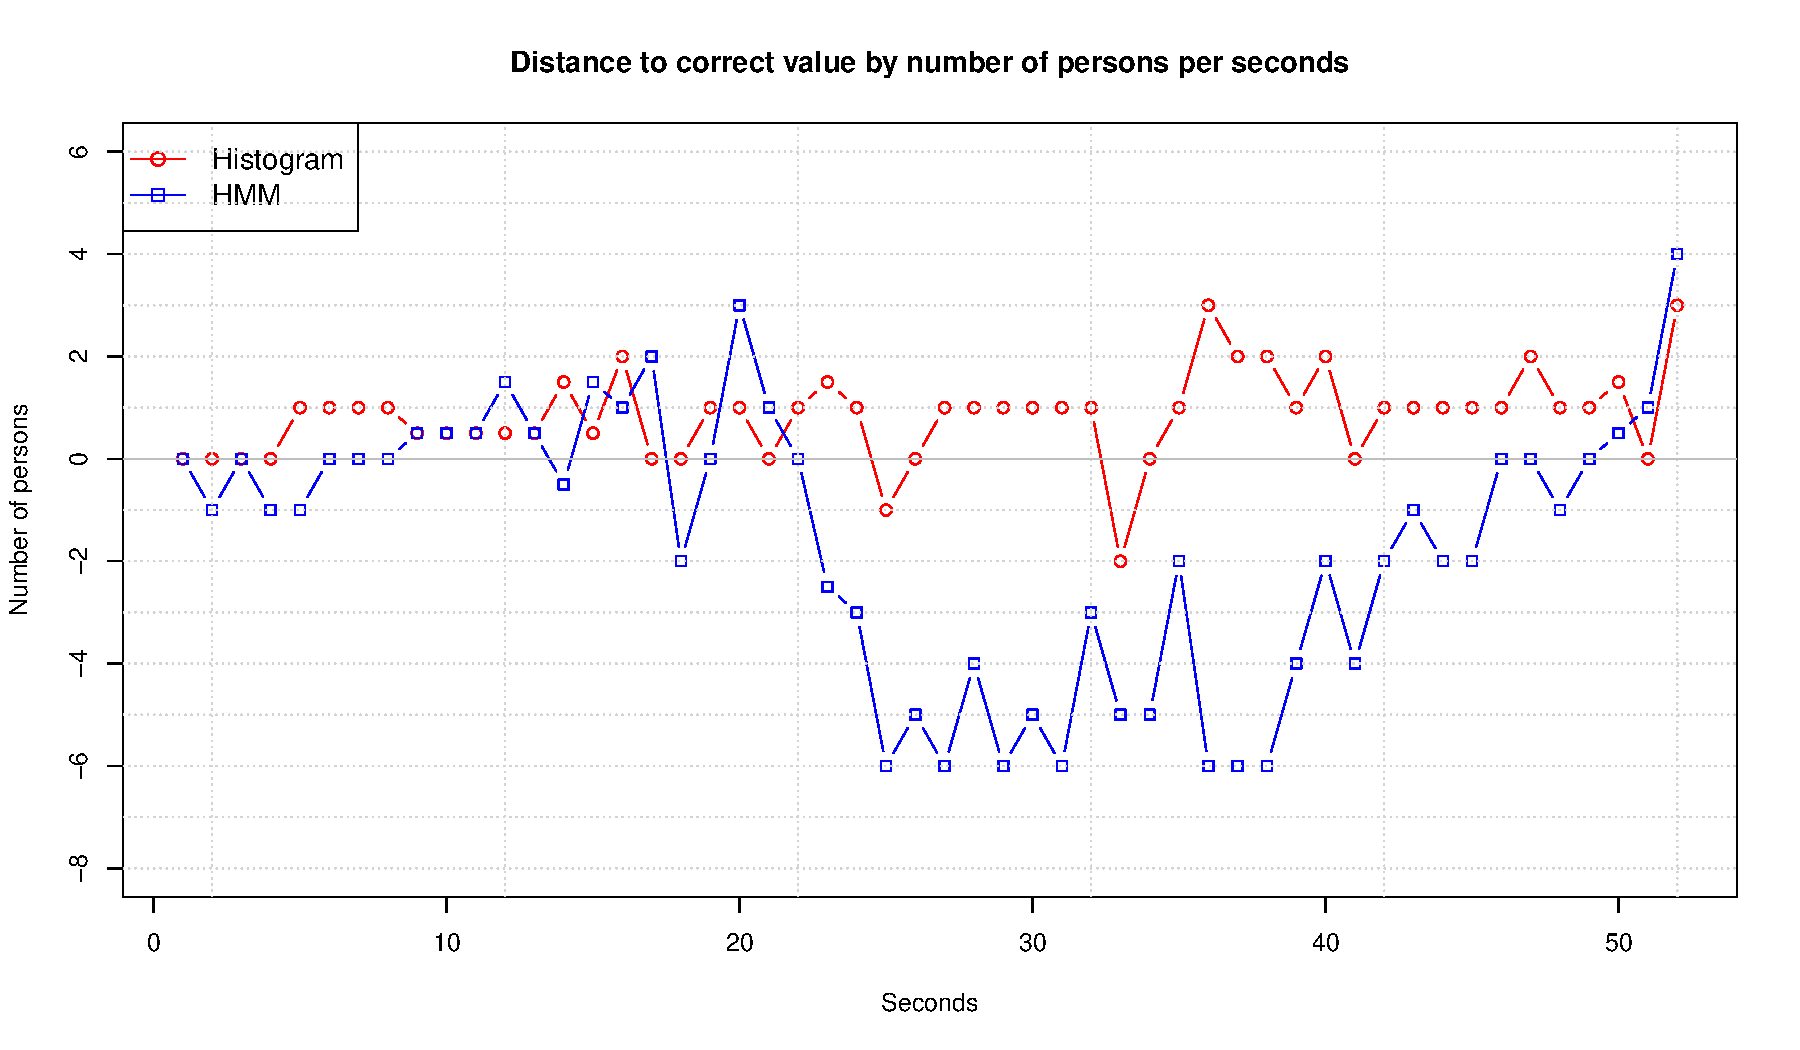
\includegraphics[width=1\textwidth]{bilder/safest_plot_innenhof_910_nolearn.pdf}
\caption{Innenhof: Histogramm vs. nicht lernendes HMM}
	\label{fig:Innenhof_nl}
\end{figure}
\begin{figure}
	\centering
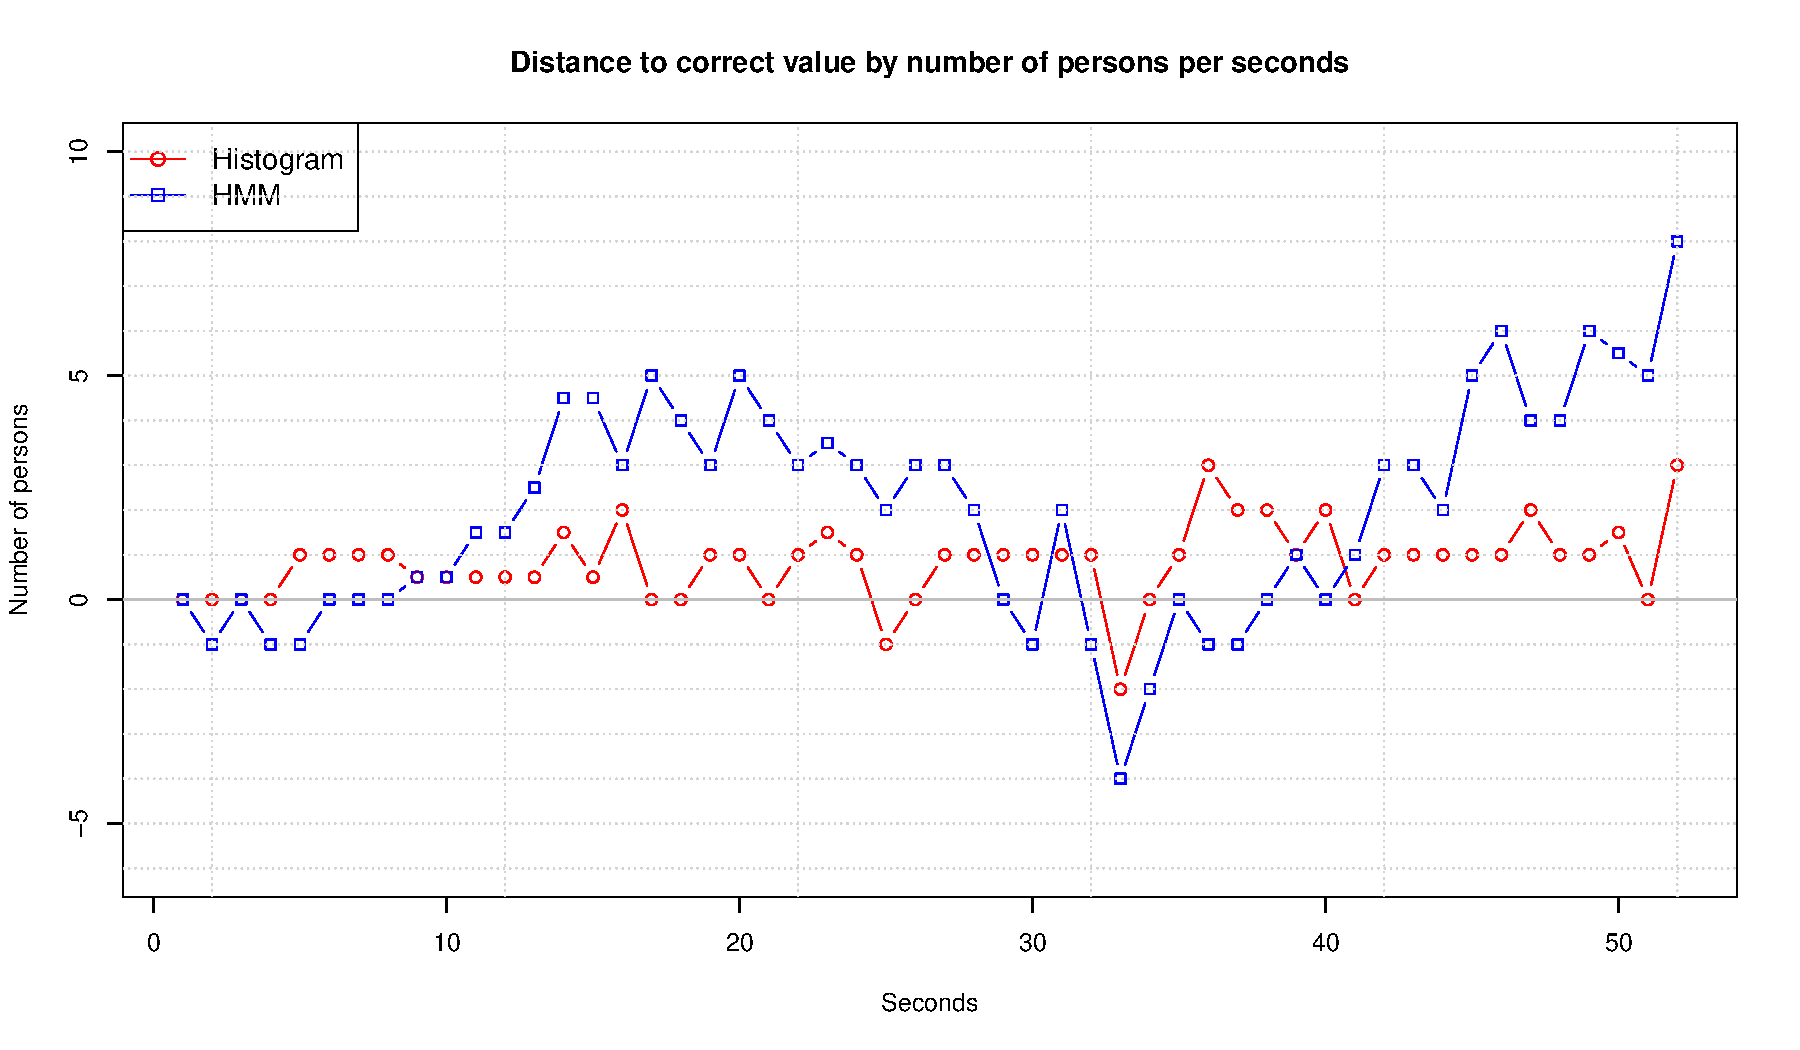
\includegraphics[width=1\textwidth]{bilder/safest_plot_innenhof_910_learn.pdf}
\caption{Innenhof: Histogramm vs. nicht lernendes HMM}
	\label{fig:Innenhof_nl}
\end{figure}
In beiden Grafiken sieht man, dass der Histogramm-basierte Algorithmus für dieses Video bessere Ergebnisse liefert, als der HMM-basierte Algorithmus.\\
Allerdings ist der HMM-basierte Algorithmus mit Lernen besser als ohne Lernen.

\subsection{Vergleich mit Histogramm-basierter Implementierung: Eingang}
\label{sec:eval_eingang}
\begin{figure}
	\centering
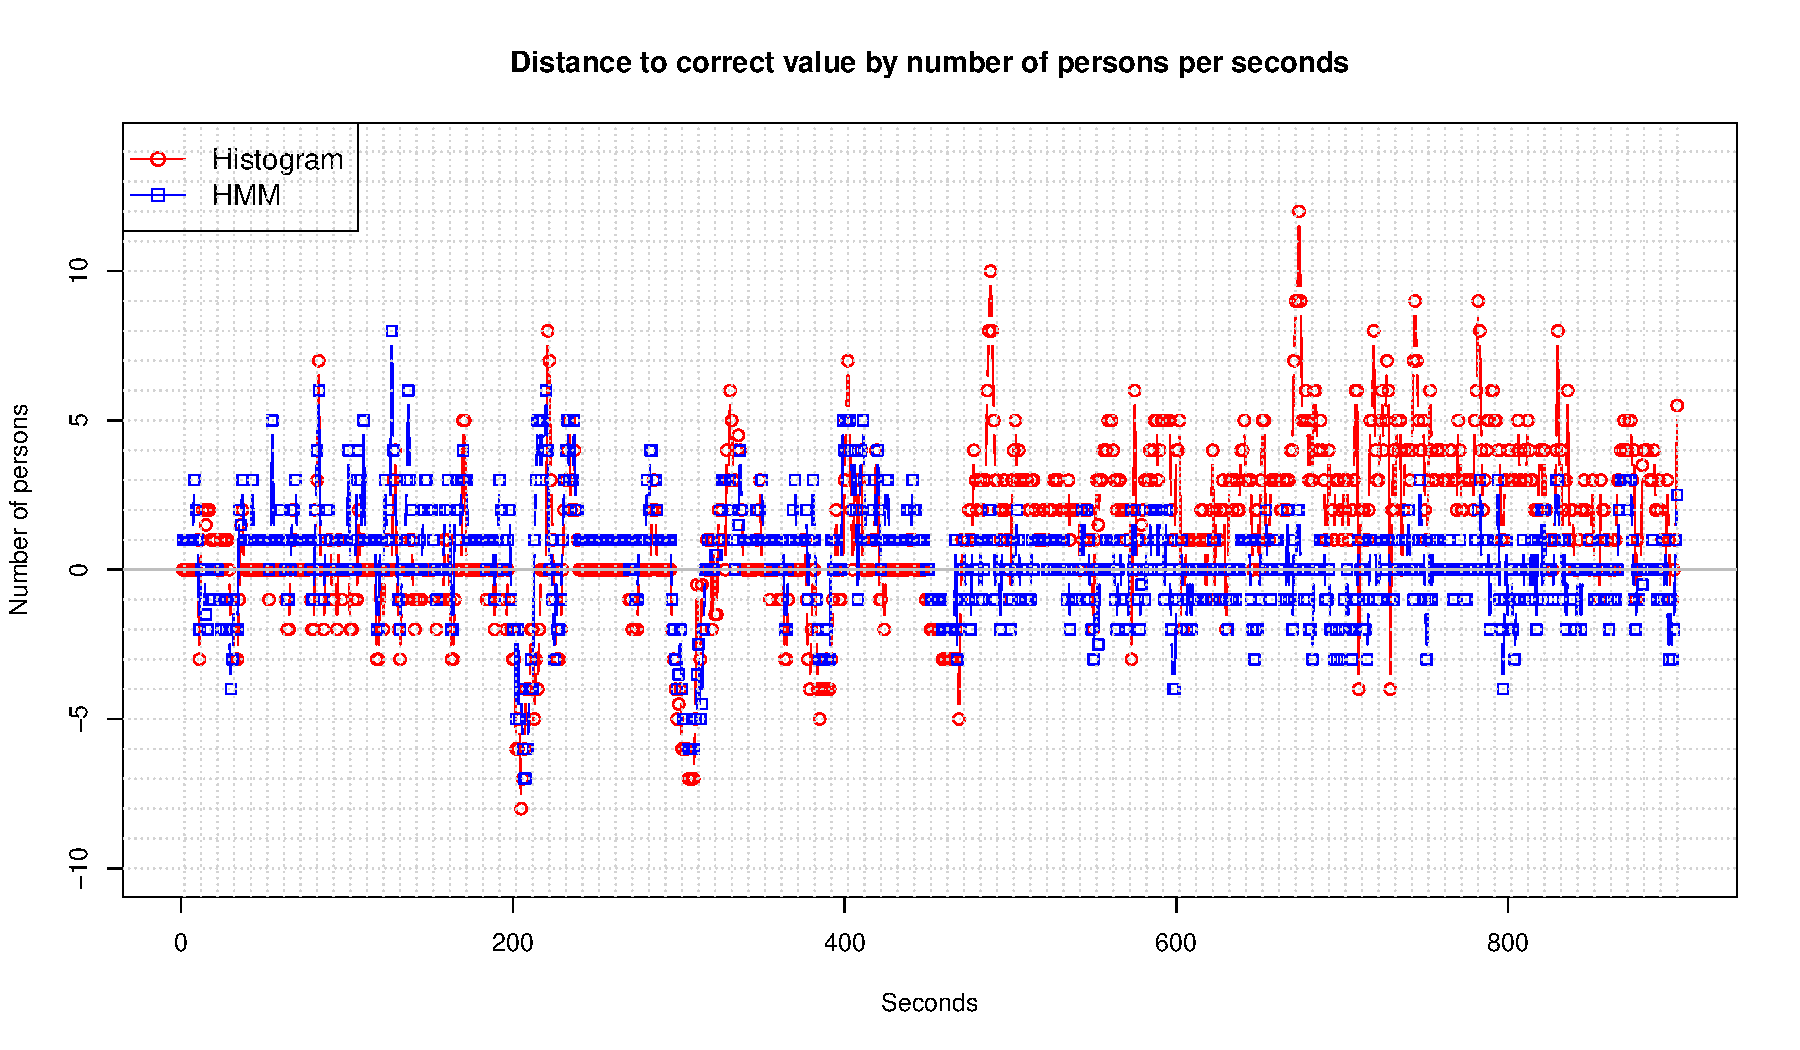
\includegraphics[width=1\textwidth]{bilder/safest_plot_eingang2_nolearn.pdf}
	\caption{Eingang: Histogramm vs. nicht lernendes HMM}
	\label{fig:Eingang-nolearn}
\end{figure}
\begin{figure}
	\centering
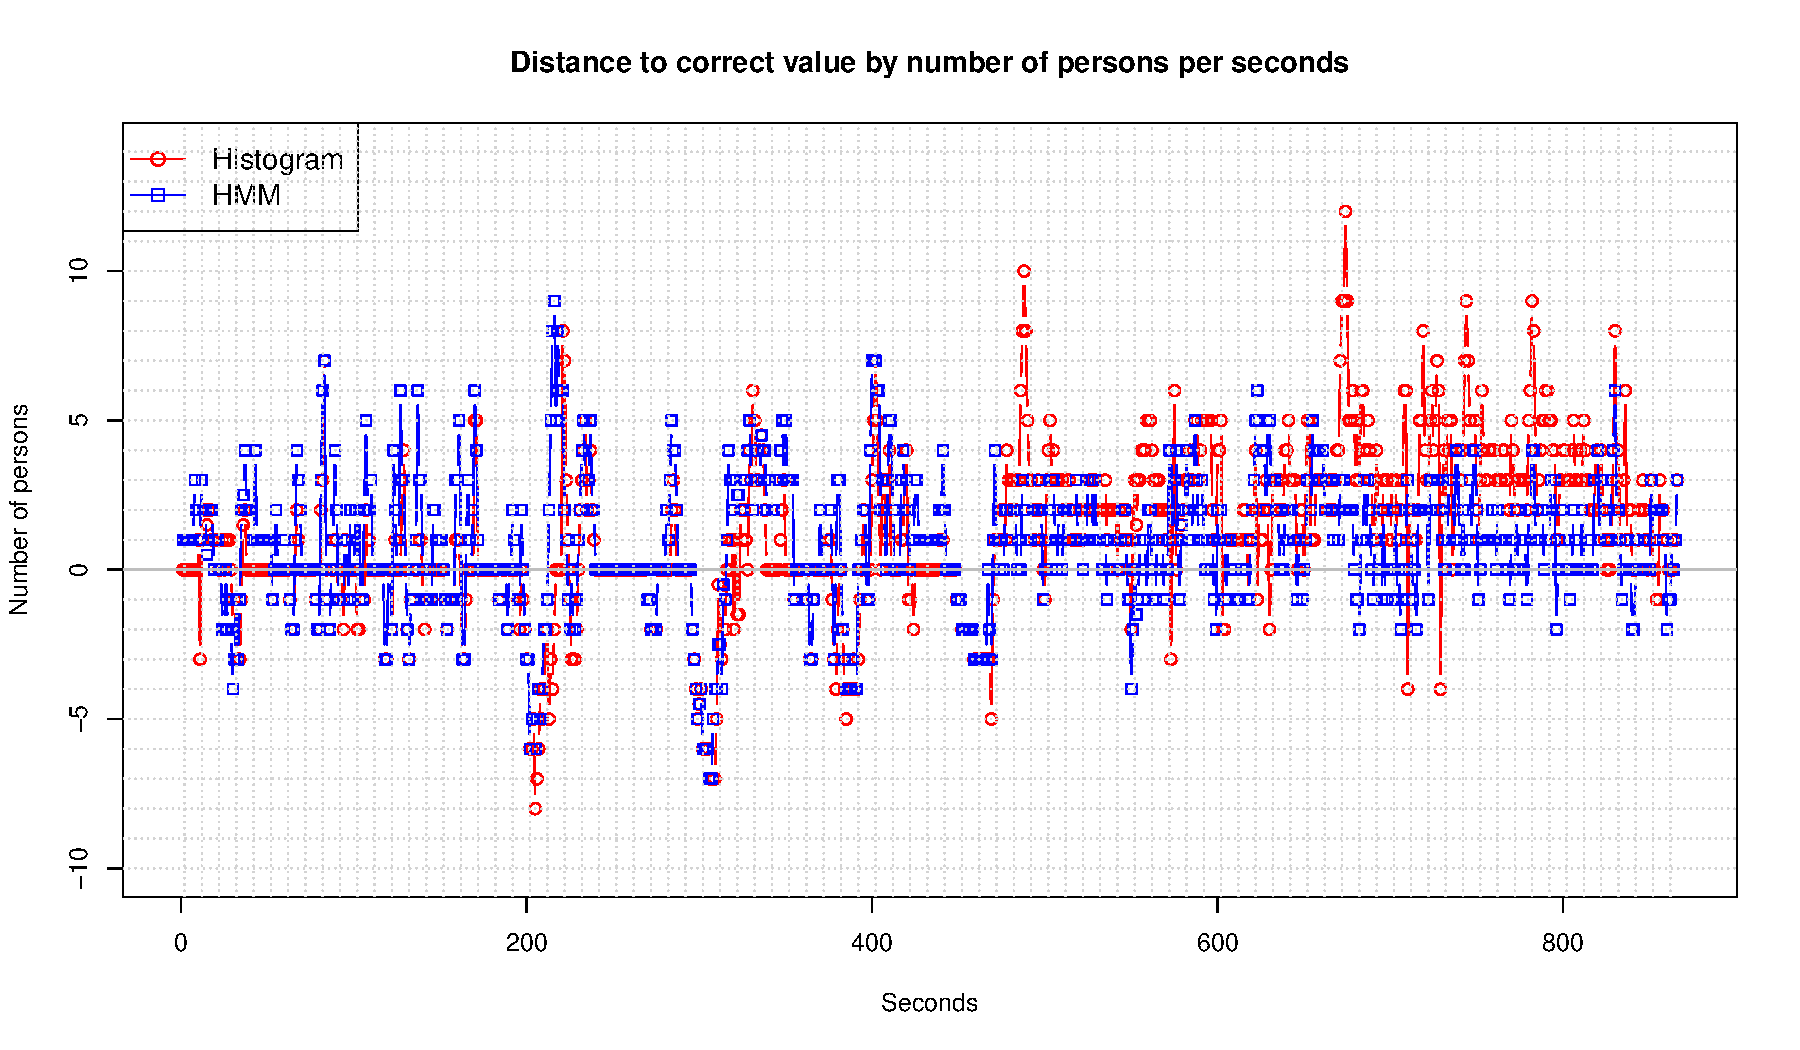
\includegraphics[width=1\textwidth]{bilder/safest_plot_eingang2_learn.pdf}
	\caption{Eingang: Histogramm vs. nicht lernendes HMM}
	\label{fig:Eingang-learn}
\end{figure}
In der Grafik \ref{fig:Eingang-nolearn} kann man sehen, dass beide Algorithmen Probleme mit dem Videomaterial haben. Was auch auffällt ist, dass gerade in der zweiten, schlechteren Hälfte der HMM-basierte Algorithmus deutlich bessere Ergebnisse liefert, als der Histogrammbasierte Algorithmus.\\
In Grafik \ref{fig:Eingang-learn} ist zu sehen, dass der HMM-basierte Algorithmus anfangs eine höhere Varianz aufweist, aber in der zweiten Hälfte des Videos dichter an den korrekten Werten liegt.


\subsection{Vergleich mit Histogramm-basierter Implementierung: Tegel}
\label{sec:eval:tegel}
\begin{figure}
	\centering
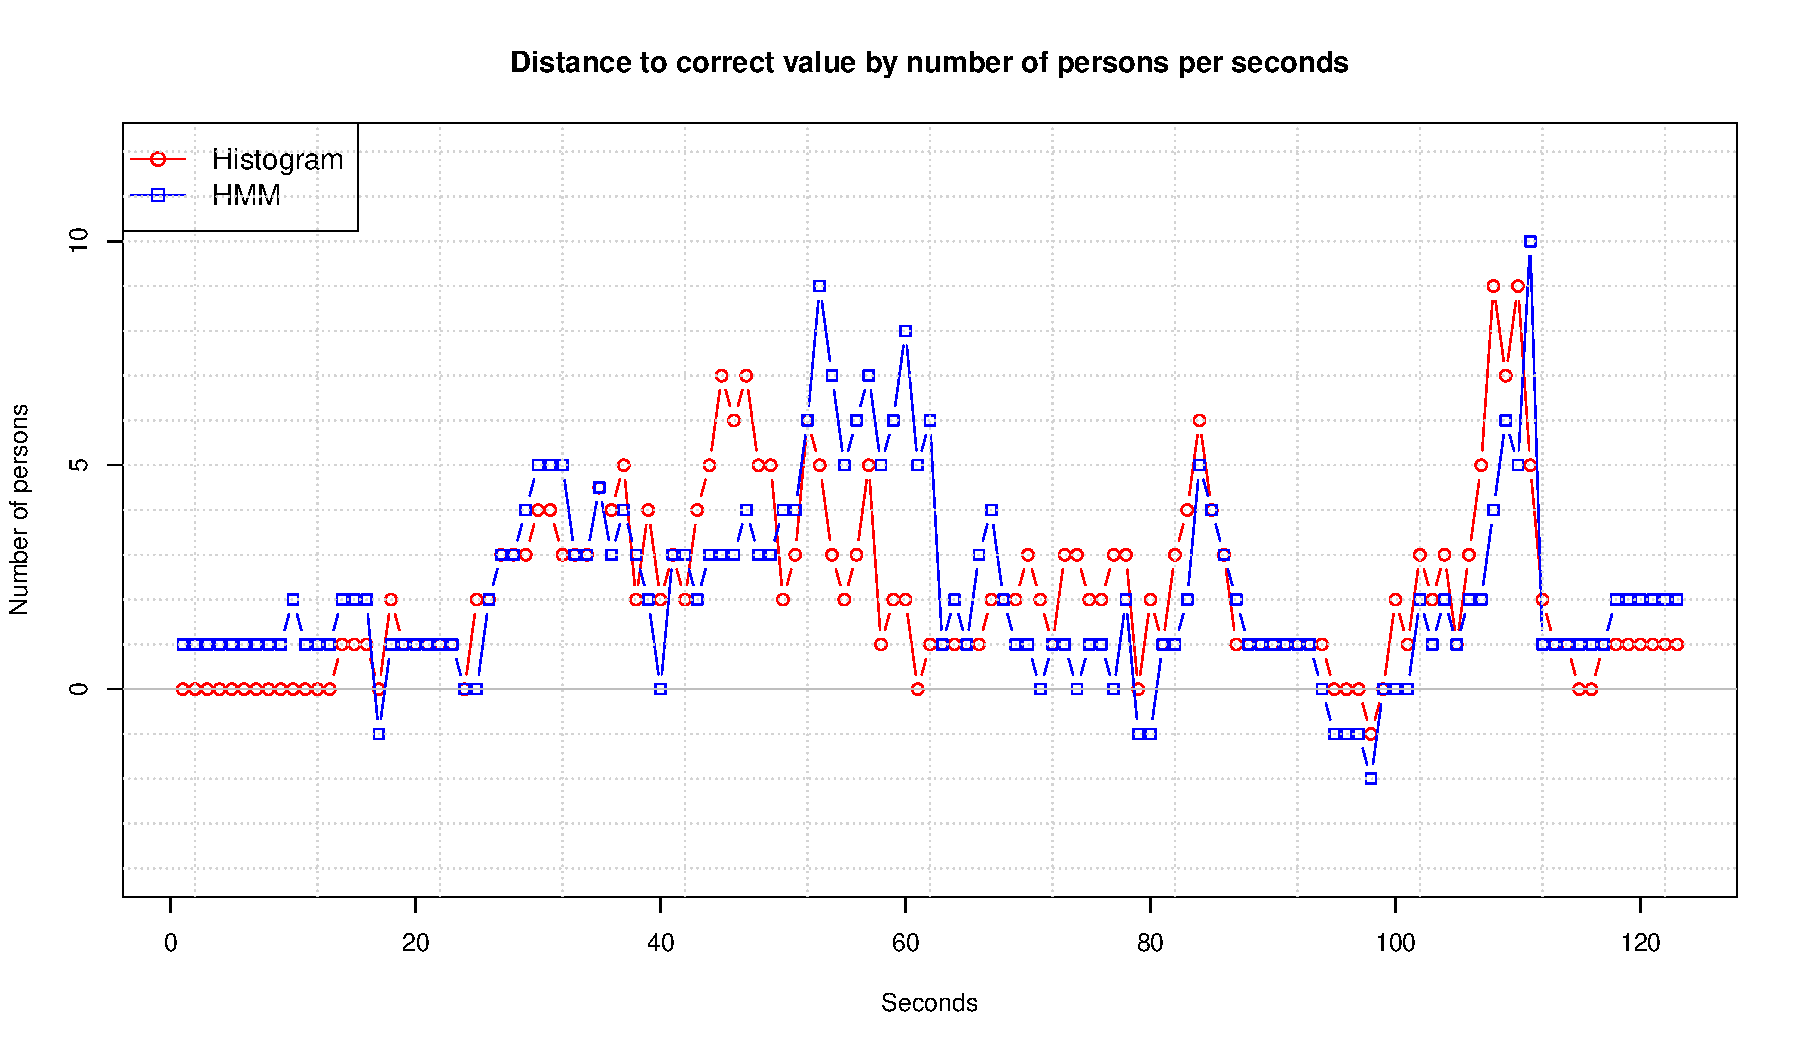
\includegraphics[width=1\textwidth]{bilder/safest_plot_tegel_7-55_hmm_learn.pdf}
	\caption{Tegel: Histogramm vs. lernendes HMM}
	\label{fig:tegel_7-55_learn}
\end{figure}

\begin{figure}
	\centering
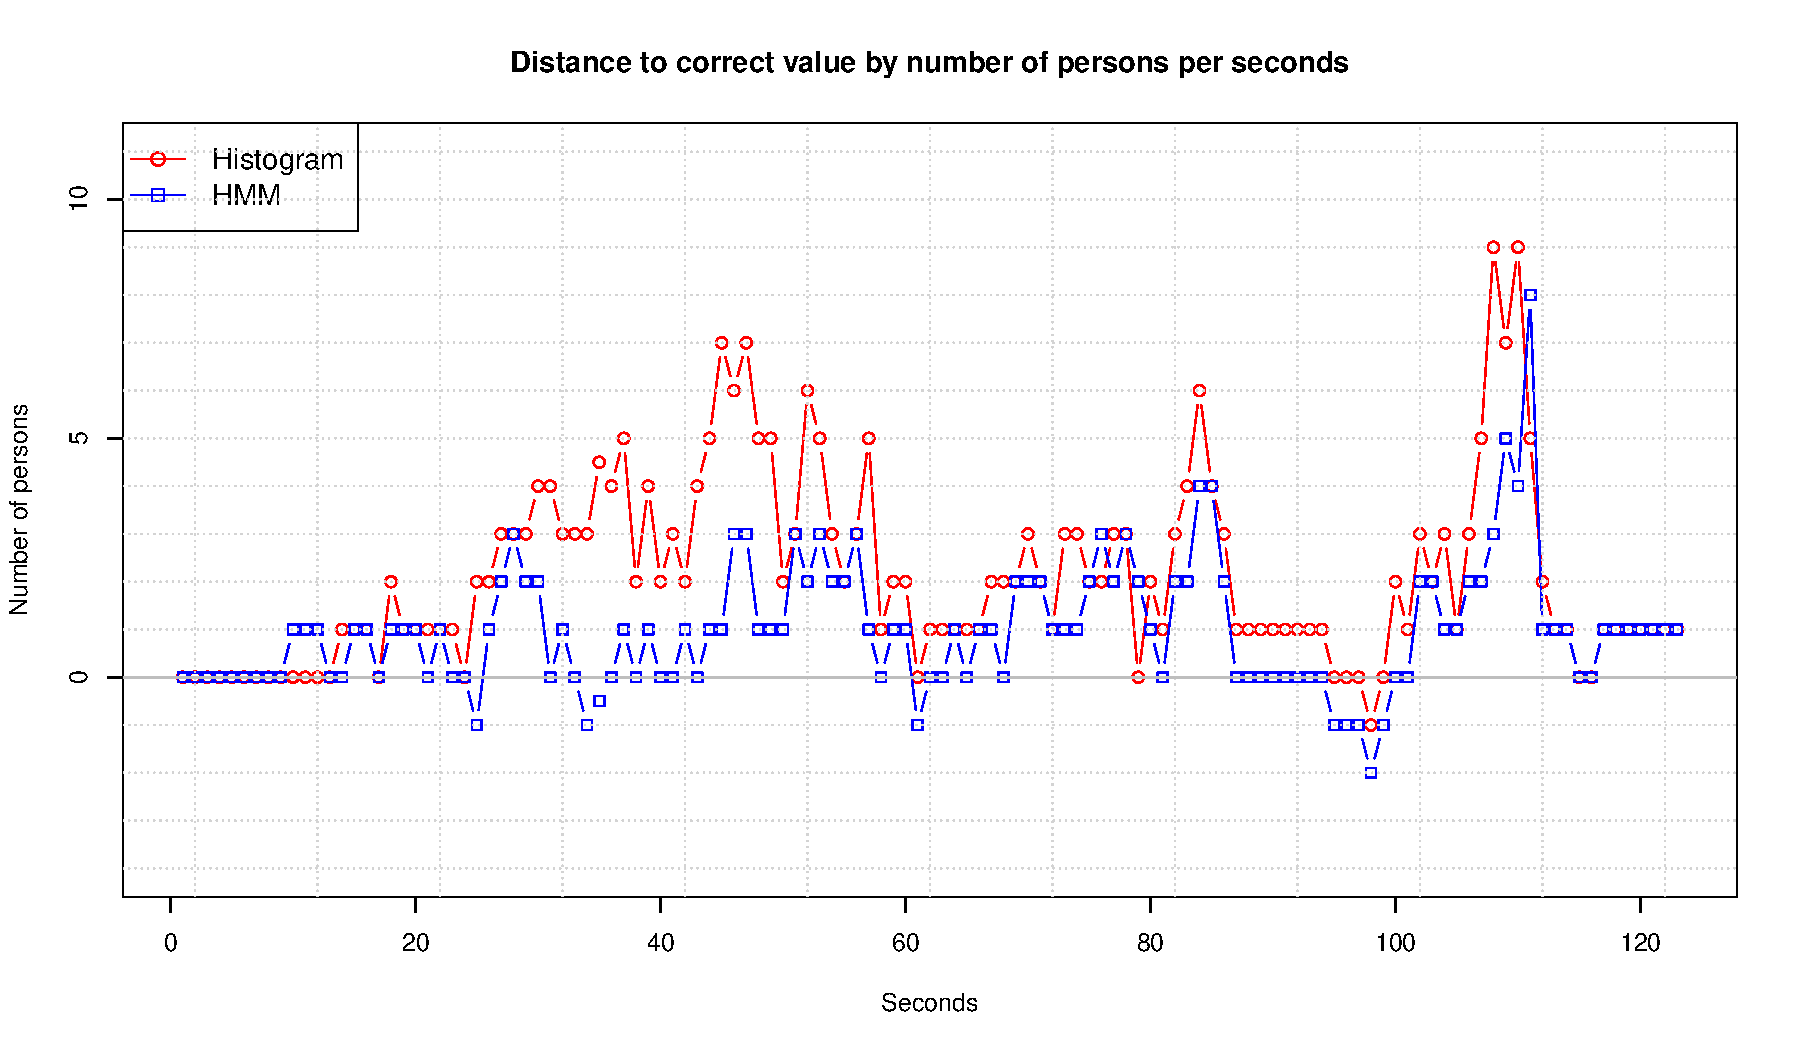
\includegraphics[width=1\textwidth]{bilder/safest_plot_tegel_7-55_hmm_nolearn.pdf}
	\caption{Tegel: Histogramm vs. HMM mit generischen Startwerten}
	\label{fig:tegel_7-55_nolearn}
\end{figure}
Wie man Abbildung \ref{fig:tegel_7-55_learn} entnehmen kann, sind die Ergebnisse beider Algorithen vom Verlauf her sehr ähnlich. Im Großen und Ganzen kann man den Histogramm-basierten Algorithmus dem von uns entwickten HMM-basierten Algorithmus gegenüber im Falle dieses Videos als überlegen betrachten.
Allerdings haben beide Algorithmen relativ starke Abweichungen gegenüber den eigentlich gezählten Werten (HMM maximal 10, Histogramm maximal 9).
Es fällt weiterhin auf, dass der HMM-basierte Algorithmus zwischenzeitlich immer wieder bessere Ergebnisse liefert (z.B. bei ca. 40-50 Sekunden und bei ca. 70-80 Sekunden).
Dies liegt vermutlich daran, dass die HMMs zu diesem Zeitpunkt gerade eine Lernphase abgeschlossen haben, deren Ergebnis für eine gewisse Zeit andauert, so dass das HMM die Wirklichkeit in diesen Momenten besser beschreibt.\\
Eine weitere Auffälligkeit ist, dass das für dieses Video ein nicht lernendes HMM mit generischen Werten bessere Ergebnisse liefert, als das lernende HMM und das Histogramm-basierte (vergleiche Grafik \ref{fig:tegel_7-55_nolearn}.

\subsection{Diskussion}
\label{sec:diskuss}

Zu erkennen an den beschreibung der vorangehenden graphiken ist das....

%TODO:
 %bezug auf anforderungen nehmen, punkte erfüllt?
 %hmm topologie?
 %andere libs?
 %forward vs. viterbi
 %dynamische histrogramm/cluster grenzen für dc wert in zukunft?
 %viterbi/forawrd gibt zustand, man kann entweder gewichtestes würfeln oder aber deterministisch die wahrschienlichste beobachtung nehmen, was ist besser? -> test?
 %performance gewinn durch threading zusätzlich
Lerndauer vermutlich zu kurz, daher stellt sich das HMM nie richtig ein und es kommt zusätzlich zu Effekten wie Ghosting.

Der Vergleich der Algorithmen bezieht sich rein auf das Ergebnis der Hintergrder Algorithmen bezieht sich rein auf das Ergebnis der Hintergrundentfernung.
Im Bezug auf Performance ist der Histogramm-basierte Algorithmus wesentlich besser (ca. 3-4 Frames/sec vs. ca 20-25 Frames / sec).

Größte Performance-Bremse lt. Callgrind: der .at(foo, bar): Zugriff auf einzelne Elemente des Arrays.

\subsection{CvHMM}
\label{sec:CvHMM}
Leider hat sich im Laufe des Projekts gezeigt, dass CvHMM leider sehr ineffizient auf einzelne Daten zugreift.\\

Ein weiterer großer Nachteil von CvHMM ist, dass nur der Baum-Welch-, der Viterbi- und der Decode-Algorithmus angeboten werden.
 Gerade hier ist wiederum ein Manko zu sehen, da wir später den Forward-Algorithmus gebraucht hätten und nun stattdessen den Viterbi-Algorithmus verwenden müssen, der jedoch ineffizienter als der Forward-Algorithmus ist.

Zusammenfassend lässt sich zur Wahl der HMM Bibliothek sagen, dass es wohl das Ergebnis des Projekts erheblich hätte verbessern können, wenn unsere Wahl auf eine andere Bibliothek gefallen wäre.

Mögliche Kandidaten zum Testen wären dabei HMMlib oder vielleicht sogar die, wie wir später herausgefunden haben, in OpenCV enthaltenen HMM-Funktionen, die allerdings innerhalb des OpenCV-Projekts nicht weiterentwickelt werden und derzeit des Status “deprecated” haben.
